\subsection{Generative Adversarial Networks}
\label{gans}
\begin{comment}

    -look at gradient descent --> adjust weights in specific direction, move down the gradient
    - discriminator (classifier) (supervised learning) (0-1) fake or real?
        --> if discriminator says fake -> negative reward for generator
    - generator (random noise) -> generates new sample
    --> competetive game (one wants error rate to be high - one wants it to be low)

    - as the descriminator gets better, the generator has to get better aswell
\end{comment}

Another adversarial framework was developed by Ian J. Goodfellow et al. \cite{gansgoodfellow2014generative} in 2014, namely Generative Adversarial Networks (GANs). 
In an opposing setup, two agents are trained simultaneously: a generative network $G$ and a discriminatory network $D$. \\
$G$ captures a predetermined training set and generates new samples from it. $D$ has the task of estimating whether the example given to it was generated by $G$ or is an original from the training set. The task of $G$ is that $D$ makes as many errors as possible, i.e. to fool $D$.\\
Goodfellow et al. used as a metaphor:
\begin{quote}
\textit{"The generative model can be thought of as analogous to a team of counterfeiters, trying to produce fake currency and use it without detection, while the discriminative model is analogous to the police, trying to detect the counterfeit currency"}, \cite{gansgoodfellow2014generative}
\end{quote}{}
\\
%In other words, G and D play a minmax game.
\\
\begin{comment}


\begin{align}
\label{gans_value_func}

\end{align}

\begin{figure}[H]
  \centering
    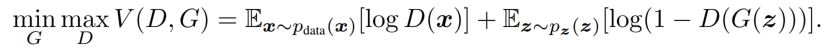
\includegraphics[width=0.9\textwidth]{adversarial_learning/images/minmax_gan.JPG}
    \label{fig:sumo}
    %\caption{Wird noch ersetzt durch Formel in Text}
\end{figure}
\end{comment}
\\
This framework is a zero-sum game (section \ref{zerosumgames}). A unique solution exists when $G$ uses the training set repeatedly and $D$ rates each sample 50/50 original/fake.\\
Both networks use backpropagation, so the generator becomes better at producing samples and the discriminator becomes more effective at detecting counterfeits.
\\
\inline{bild? und quelle medium checken!}
%https://towardsdatascience.com/explained-a-style-based-generator-architecture-for-gans-generating-and-tuning-realistic-6cb2be0f431
GANs have now been deployed in several areas. For example in the field of video gaming, where textures are edited and reproduced \cite{resolutionGANWang2018Sep} or in the domain of astrophysics, features are recovered in astronomical images \cite{astroGANSchawinski2017Feb}.\\
Another very interesting application of GANs is the \textit{Style-Based Generator Architecture} developed by Karras et al. of NVIDIA \cite{nvidiaThisPersonDoesNotExistKarras2018Dec}. They extended GANs with style transfer and designed an AI that generates deceptively real images of faces that don't really exist. The generator automatically learns to distinguish and classify different aspects of the image (\textit{styles}) without human supervision, such as pose, identity, freckles or hair). This approach not only allows a better insight into the output produced, but also delivers state-of-the-art results - high-resolution images that look more authentic than previously generated images.
%hier weiterführen GANS --> dann überleitung zum vergleich schaffen